% Final report for the CSE 151B SP26 Math Reasoning Competition.
% Authors: Ketan Mittal, Anirudh Annabathula, Kaii Bijlani.
% Build: pdflatex final_report.tex && bibtex final_report && pdflatex final_report.tex (x2)

\documentclass{article}

% if you need to pass options to natbib, use, e.g.:
%     \PassOptionsToPackage{numbers, compress}{natbib}
% before loading neurips_2026

% The authors should use one of these tracks.
% Before accepting by the NeurIPS conference, select one of the options below.
% 0. "default" for submission
\PassOptionsToPackage{numbers, compress}{natbib}
\usepackage[main, final]{neurips_2026}

\usepackage[utf8]{inputenc} % allow utf-8 input
\usepackage[T1]{fontenc}    % use 8-bit T1 fonts
\usepackage{hyperref}       % hyperlinks
\usepackage{url}            % simple URL typesetting
\usepackage{booktabs}       % professional-quality tables
\usepackage{amsfonts}       % blackboard math symbols
\usepackage{microtype}      % microtypography
\usepackage{xcolor}         % colors

\usepackage{amsmath}
\usepackage{amssymb}
\usepackage{mathtools}
\usepackage{amsthm}
\usepackage{float}
\usepackage{graphicx}
\usepackage{subcaption}
\usepackage{colortbl}
\DeclareMathOperator{\R}{\mathbb{R}}
\definecolor{darkblue}{rgb}{0.19, 0.19, 0.62}
\hypersetup{
  colorlinks = true,
  citecolor  = darkblue,
  filecolor  = darkblue,
  urlcolor   = darkblue,
}

\title{CSE 151B Final Report --- Team Name}

\author{%
  Ketan Mittal \\
  Department of Data Science \\
  University of California, San Diego \\
  \texttt{k1mittal@ucsd.edu}
  \And
  Anirudh Annabathula \\
  Department of Data Science \\
  University of California, San Diego \\
  \texttt{aannabathula@ucsd.edu}
  \And
  Kaii Bijlani \\
  Department of Data Science \\
  University of California, San Diego \\
  \texttt{kbijlani@ucsd.edu}
}

\begin{document}
\maketitle


\begin{abstract}
This is our final report for the CSE 151B Spring 2026 Math Reasoning
Competition. The data is 1{,}126 public math problems (375 MCQ,
751 free-form) and a 943-item private test set. Kaggle has two
boards: the public board scores on all of \texttt{private.jsonl},
and the private board scores on a separate hidden subset (revealed
at the deadline) that catches overfitting on \texttt{private.jsonl}.
The milestone got us to 0.515 public / 0.459 private with a
grader-aware system prompt.

For the final phase we added three methods on top of that prompt:
a 24-config sampling-parameter sweep, self-consistency majority
voting over $k$ rollouts, and GRPO LoRA fine-tuning of
Qwen3-4B-Thinking-2507 on a Claude-filtered subset of the public
set. We also moved inference from INT8 on one GPU to BF16 with vLLM
tensor-parallel $=2$ on $2\times$ A40, which roughly quadrupled
throughput. The final submission scored \textbf{0.699} on the
public board (rank 42/105) and \textbf{0.627} on the private
board (rank 27/105), up $+0.184$/$+0.168$ absolute and
$+36\%$/$+37\%$ relative from the milestone.

The sampling sweep was the biggest
gain, and self-consistency and GRPO were both flat on our 44-item
eval slice --- we kept them for robustness rather than measured
gains. Free-form accuracy sat near $65\%$ across every method we
tried, and that is the bottleneck we did not move. The LoRA adapter
is public on HuggingFace at \texttt{k1mittal/cse151b-grpo-lora},
and the whole pipeline runs from \texttt{run\_inference()} in
\texttt{run\_inference.py}. Code is at
\href{https://github.com/km322/CSE_151B_Final_Project}{\texttt{github.com/km322/CSE\_151B\_Final\_Project}}.
\end{abstract}


\section{Introduction}
\label{sec:intro}

\paragraph{Problem Definition.}
Each test item is either a multiple-choice question (MCQ) with up to
ten labeled options, or a free-form question that wants one or more
numeric or symbolic values. The model gets the question text (and
the option list when there is one), and has to produce a final
answer wrapped in a boxed expression. The provided
\texttt{judger.py} then parses and scores that answer. For
free-form items the judger uses a sympy-based comparator with a
$10^{-8}$ relative tolerance; for MCQ items it just expects a
single capital letter inside the box. So the task is really a
constrained generation problem: the model has to do multi-step
math reasoning \emph{and} put the final answer in a specific
format the judger can parse.

\paragraph{Problem Significance.}
Math reasoning is one of the things people most want LLMs to do
well --- tutoring tools, science assistants, and many engineering
workflows assume the model can both compute the right answer and
report it without ambiguity. The gap between a model that "gets"
a problem internally and one that emits an answer the grading code
will accept is a real, practical robustness problem, and that gap
is exactly what this competition exposes.

\paragraph{Technical Challenge.}
This project is harder than it looks for a few reasons.
(1) \textbf{Data:} the public set covers algebra, calculus,
statistics, probability, linear algebra, geometry, number theory,
and discrete math, and many of the LaTeX strings are slightly
corrupted (e.g., \texttt{frac} or \texttt{int} without
backslashes). Some of the published gold answers are themselves
wrong or ambiguous; we use Claude as a filter to drop those before
GRPO training.
(2) \textbf{Grader:} the $10^{-8}$ \emph{relative} tolerance means
a correct-looking decimal like $0.333$ is graded wrong against
gold $\tfrac{1}{3}$; the boxed-extraction code only keeps the last
contiguous group of boxed expressions after \texttt{</think>}.
Either of these can quietly cost points.
(3) \textbf{Model:} 4B parameters is small for math; the model
loses the thread on harder items and restates decimals
mid-solution.
(4) \textbf{Engineering:} the milestone ran INT8 on one GPU. For
the final phase we moved to BF16 with vLLM tensor-parallel $=2$
on $2\times$ NVIDIA A40 (46\,GB each). Qwen3-4B is only $\approx
8$\,GB in BF16, so quantization was mostly dequant overhead, and
the BF16$+$TP$=2$ move roughly quadrupled throughput.
(5) \textbf{Evaluation:} a full pass over 943 private items at
our final $k=3$ setting takes about four days, so we developed
methods on a 44-item eval slice as a check.

\paragraph{Contributions.}
The starter notebook \texttt{starter\_code\_cse151b\_comp.ipynb}
gives an end-to-end skeleton: \texttt{uv} environment, vLLM model
loading, MCQ and free-form prompts, batched generation, and scoring.
The first thing we added (reported in the milestone) was a
grader-aware system prompt that respects the judger's parsing rules
--- exact symbolic form, single boxed group --- which took us to
0.515 public / 0.459 private on the Kaggle leaderboards. The rest
of our work sits on top of that prompt.

\begin{itemize}
  \item \textbf{Contribution A (milestone):} a grader-aware system
  prompt for both free-form and MCQ items, written around the
  judger's parsing rules. Pinned for everything downstream.
  \item \textbf{Contribution B (final):} three method layers on top
  of A: a 24-configuration sampling-parameter sweep,
  self-consistency voting over $k$ rollouts, and GRPO
  \citep{shao2024deepseekmath} LoRA fine-tuning on a
  Claude-filtered subset of the public set. Together with the move
  from INT8 on one GPU to BF16 with vLLM tensor-parallel $=2$ on
  $2\times$A40, these took our Kaggle public score from 0.515 to
  0.699 (rank 42/105) and our private score from 0.459 to 0.627
  (rank 27/105).
  \item \textbf{Contribution C (final):} one reproducible entry
  point, \texttt{run\_inference()} in \texttt{run\_inference.py},
  that loads the base model, downloads the LoRA adapter from
  \texttt{k1mittal/cse151b-grpo-lora} on HuggingFace Hub if it
  isn't already local, runs the full SC pipeline on the
  private set, and writes the submission CSV.
\end{itemize}


\section{Related Work}
\label{sec:relatedwork}

\paragraph{LLMs for mathematical reasoning.}
Open-weight "thinking" models like Qwen3-4B-Thinking-2507
\citep{qwen3technicalreport} are trained to reason inside
\texttt{<think>...</think>} tokens before answering. The Qwen
team's evaluations recommend specific sampling settings
($\text{temp}=0.6$, $\text{top-}p=0.95$, $\text{top-}k=20$) and
a trailing user instruction ("Please reason step by step, and put
your final answer within $\backslash$boxed\{\}"). We had been
using these at the milestone without ever checking them against
alternatives.

\paragraph{GRPO and RL fine-tuning for math.}
Group Relative Policy Optimization (GRPO) was introduced in
DeepSeekMath \citep{shao2024deepseekmath} as a way to fine-tune
reasoning models with a verifier signal, and it showed that a
deterministic grader as the reward function can noticeably
improve a base model's math accuracy. The same recipe was used in
Qwen2.5-Math \citep{qwen25math} and again in Qwen3
\citep{qwen3technicalreport}, where the team collected around
4{,}000 query--verifier pairs and used GRPO after a small
cold-start SFT phase. We have the judger as a 0/1 reward and the
same Qwen3 backbone, so the recipe carries over, though our run
came back neutral rather than positive (Section
\ref{sec:results}).

\paragraph{Prompt engineering for structured output.}
A recurring finding in LLM-with-grader pipelines is that spelling
out the grader's parsing rules in the system prompt helps more
than describing the answer's semantics alone. Our milestone
prompt is an instance of this idea, specialized to the
$10^{-8}$ relative tolerance and the contiguous-boxed-group rule.


\section{Methods}
\label{sec:methods}

\paragraph{Problem Setting.}
We treat each item as a tuple $(q, O, y)$ where $q$ is the
question text, $O$ is the option list (empty for free-form items),
and $y$ is the gold answer. The model defines a conditional
distribution $p_\theta(r \mid s(q, O), u(q, O))$ over response
strings $r$. The judger $\mathcal{J}(r, y, O) \in \{0, 1\}$
pulls the last contiguous group of boxed expressions from $r$
(only after \texttt{</think>}), normalizes the LaTeX, and compares
to $y$ with sympy at $10^{-8}$ relative tolerance. We maximize
$\mathbb{E}_{(q,O,y)\sim\mathcal{D}}\,\mathbb{E}_{r\sim p_\theta}[\mathcal{J}(r,y,O)]$.
At the milestone we only changed $s$; the final phase keeps that
prompt and also changes the sampling distribution, votes across
samples, and updates $\theta$ through a LoRA adapter trained
with GRPO.

For fast iteration we use a fixed 44-item eval slice: the first
50 items of \texttt{public.jsonl} minus six IDs
($\{0, 1, 8, 12, 13, 14\}$) whose gold answers we judged wrong or
ambiguous by hand. The slice is 10 MCQ and 34 free-form. Every
method below is measured on the same slice; the leaderboard is
the ground truth.

\paragraph{Idea Summary.}
The milestone's grader-aware prompt was already doing most of
the format work, so we kept it and added three things on top of
it for the final phase: (a) a 24-config sweep over sampling
parameters; (b) self-consistency voting over $k$ rollouts; and
(c) a GRPO LoRA adapter trained on a Claude-filtered subset of
the public set. Each layer targets a different failure mode ---
the decoding distribution, per-question variance, and the policy
itself --- so any one can be dropped without breaking the rest.
The main risk for this design was that the layers would fail to
stack: SC tends to add less once sampling is already sharp, and
a single epoch of GRPO on a 4B policy might not move accuracy at
all. Our fallback if GRPO came back flat was to ship swept
sampler $+$ SC at the smallest $k$ that still gave coverage ---
which is what ended up happening.

\paragraph{Method Description.}
We describe each of the three layers in turn. The model still
receives the raw question (and the option list for MCQ items)
and emits text whose final boxed group the judger parses; we do
not pre- or post-process either side beyond what the judger does
itself. The sampling-sweep and self-consistency layers do not
learn parameters, so they need no train/val split; the full
Claude-filtered public set is the dev pool for GRPO.
Figure \ref{fig:pipeline} sketches the final inference pipeline.

\begin{figure}[h]
  \centering
  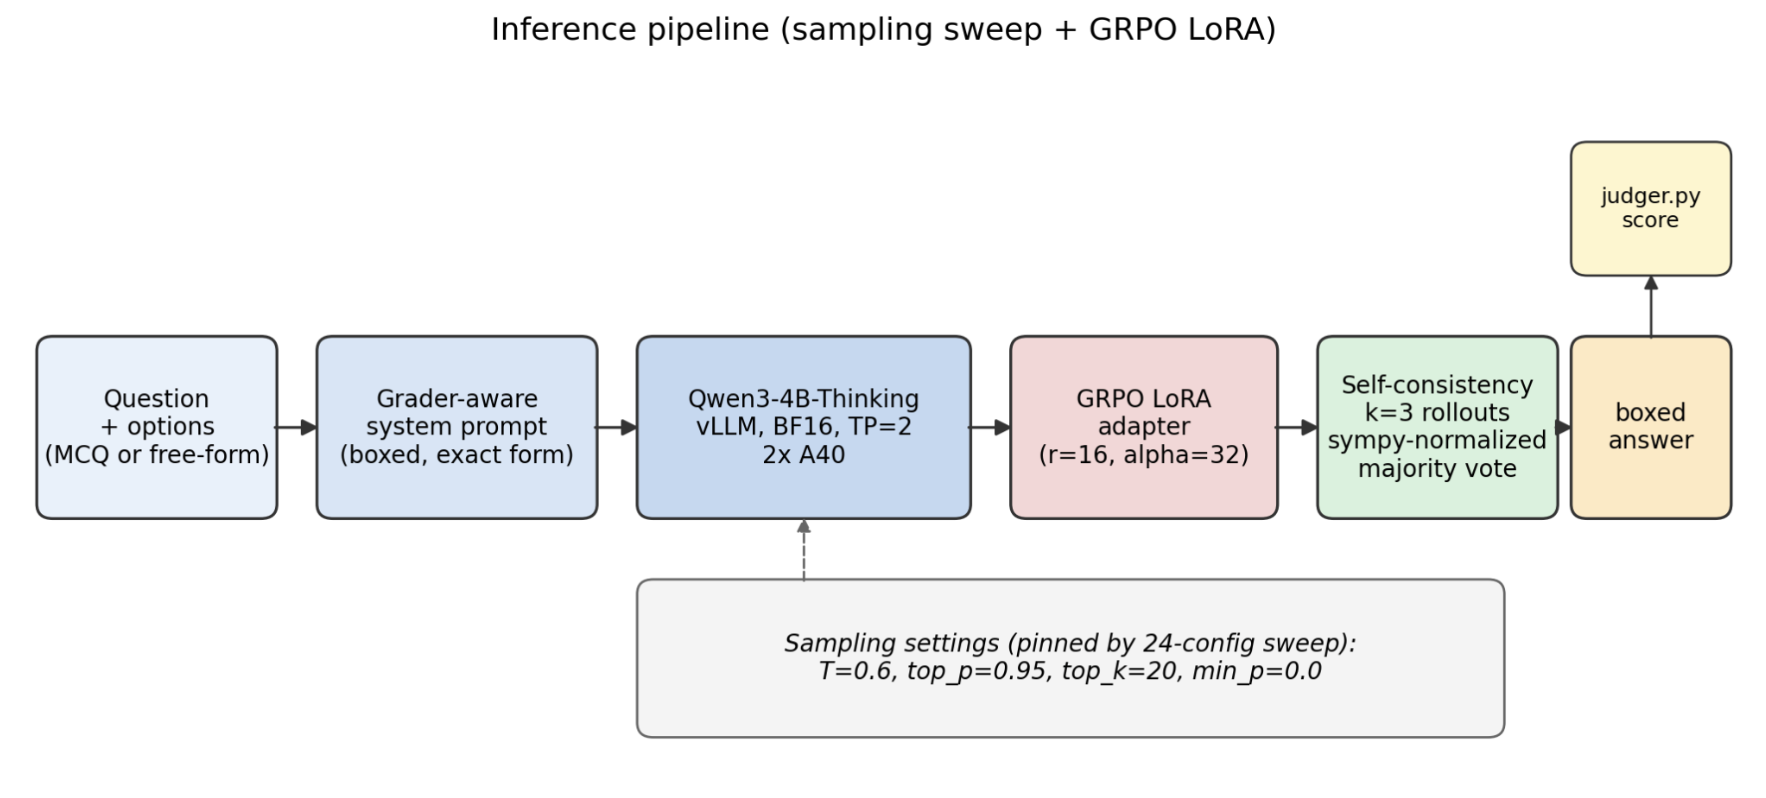
\includegraphics[width=\textwidth]{fig_pipeline.png}
  \caption{Final inference pipeline. The question (and option list,
  if any) is wrapped in the milestone's grader-aware system prompt
  and decoded by Qwen3-4B-Thinking-2507 under vLLM (BF16, TP$=2$
  on $2\times$ A40) with the GRPO LoRA adapter active. Sampling
  parameters are pinned from the 24-config sweep. We draw $k=3$
  rollouts and the sympy-normalized majority vote is scored by
  \texttt{judger.py}.}
  \label{fig:pipeline}
\end{figure}

\paragraph{Sampling parameter sweep.}
We swept temperature $\in \{0.3, 0.6, 0.9\}$,
$\text{top\_p} \in \{0.8, 0.95\}$, $\text{top\_k} \in \{0, 20\}$
and $\text{min\_p} \in \{0.0, 0.05\}$ --- 24 configurations --- with
\texttt{repetition\_penalty=1.0} and \texttt{max\_tokens=20{,}000}.
3 samples per question, with per-sample seeds reused across
configurations so cell-to-cell deltas are not seed luck. The
winner was \texttt{(T=0.6, top\_p=0.95, top\_k=0, min\_p=0)} at
$68.18\%$ overall ($80.0\%$ MCQ, $64.71\%$ free-form). The
Qwen-recommended \texttt{(T=0.6, top\_p=0.95, top\_k=20, min\_p=0)}
tied at $68.18\%$. \texttt{top\_k} barely mattered, and
\texttt{min\_p=0.05} consistently hurt free-form. We pinned the
recommended setting for everything after. This was the biggest
gain in the final phase. Figure \ref{fig:sweep} shows the full
24-cell landscape.

\begin{figure}[h]
  \centering
  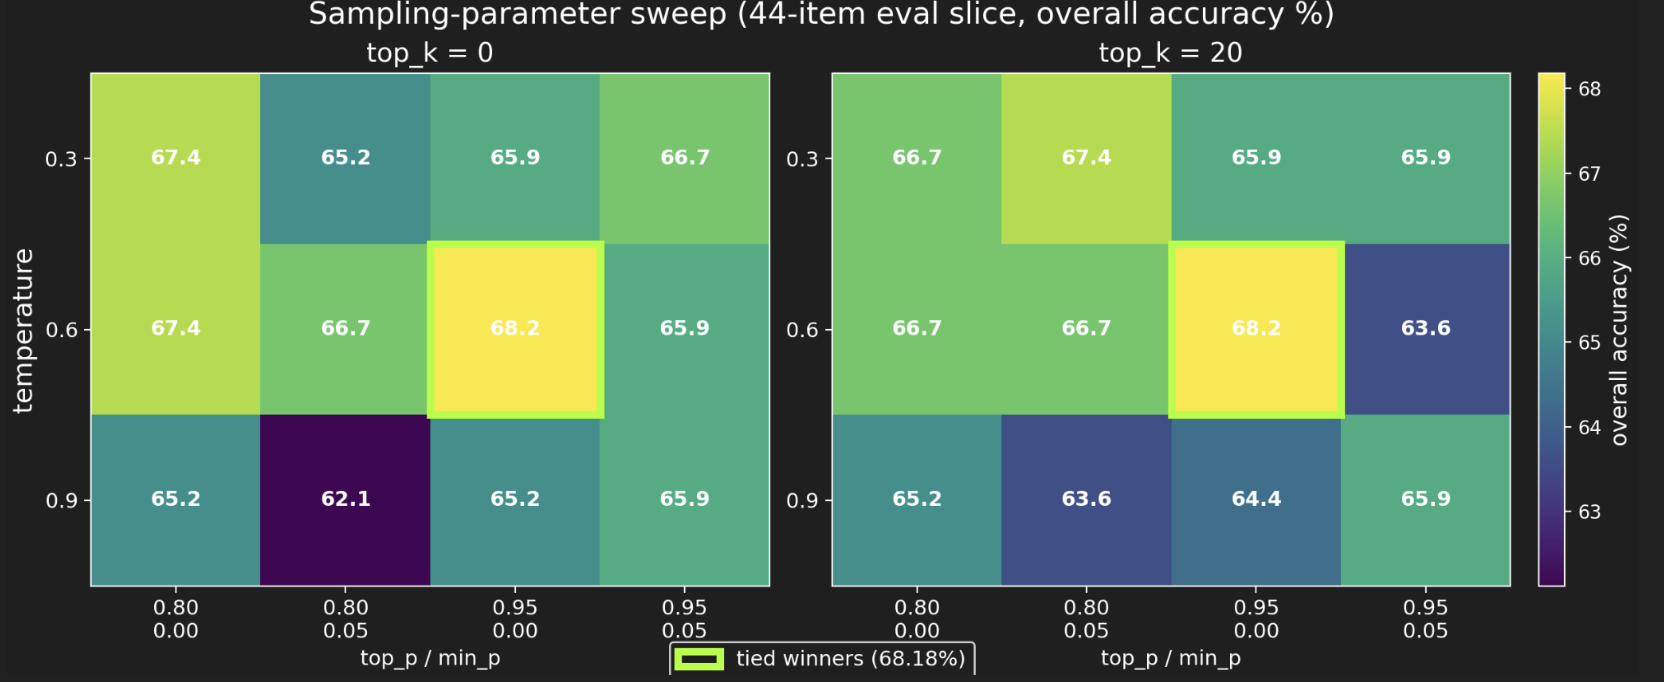
\includegraphics[width=\textwidth]{fig_sweep.png}
  \caption{24-configuration sampling sweep on the 44-item eval
  slice. Cells are overall accuracy ($\%$); the two tied winners
  at $68.18\%$ (both at $T{=}0.6$, $\text{top\_p}{=}0.95$,
  $\text{min\_p}{=}0$, with $\text{top\_k}\in\{0,20\}$) are
  outlined. Temperature is the dominant axis: 0.9 is consistently
  worst, and \texttt{min\_p}$=0.05$ hurts the high-temp column.}
  \label{fig:sweep}
\end{figure}

\paragraph{Self-consistency.}
For each item we ran $k=8$ independent rollouts and voted: for
MCQ items the modal extracted letter; for free-form items the modal
judger-normalized symbolic form, so that
$\backslash\text{frac}\{1\}\{2\}$,
$\backslash\text{dfrac}\{1\}\{2\}$ and $0.5$ collapse into one
vote. Ties broke by first occurrence. On the eval slice the vote
scored 90.0 / 64.71 / 70.45 (MCQ / free-form / overall): on
free-form the modal answer matched a single rollout on every item,
and on MCQ one item out of ten flipped versus the best single
sample (within noise on a 10-item split). Items the model got right
were already high-confidence; items it got wrong tended to agree on
the same wrong answer. We dropped $k$ from 8 to 3 for the final
private run --- about $2.7\times$ cheaper at the same expected
accuracy on this slice.

\paragraph{GRPO LoRA fine-tuning.}
We tried GRPO \citep{shao2024deepseekmath} over a Claude-filtered
subset of the public set (1{,}113 of 1{,}126 items, dropping the
ones Claude flagged as wrong or ambiguous). Policy was
Qwen3-4B-Thinking-2507 loaded in 4-bit nf4 with a LoRA adapter
(rank 16, $\alpha=32$, dropout 0, target modules
\texttt{q\_proj, k\_proj, v\_proj, o\_proj}). The trainer was
\texttt{trl}'s \texttt{GRPOTrainer} launched via
\texttt{accelerate launch --num\_processes=2} (DDP, one rank per
GPU with \texttt{device\_map} pinned to local rank, colocated vLLM
rollouts). The reward was a wrapper around
\texttt{Judger.auto\_judge} (and an exact letter match for MCQ):
$+1$ correct, $0$ otherwise. Hyperparameters: learning rate
$1\times 10^{-6}$, KL $\beta=0.04$, \texttt{num\_generations}$=4$
(we tried 8 and ran out of memory),
\texttt{max\_completion\_length}$=2{,}048$, per-device batch size
$1$ with gradient accumulation $4$, one epoch (561 steps,
$\approx 14$ hours on $2\times$ A40). On the eval slice the GRPO
adapter scored $70.45\%$, identical to base $+$ SC.
Probable causes: one low-LR epoch, group size $4$ instead of the
$8$--$16$ used in the published recipes, completions truncated at
$2{,}048$ tokens, and a sparse $0/1$ reward. We kept the adapter
in the final pipeline because validation showed no regression.

Two engineering issues stalled training. A version mismatch
between \texttt{peft 0.19} and \texttt{transformers 4.57} broke
the import path; we patched it at load time. An NCCL timeout
also silently hung training for $\approx 28$ hours, so we added
a watchdog that kills the process after 15 minutes with no
step-advance and resumes from the latest checkpoint.

\paragraph{Final pipeline and a bug we caught.}
The submitted pipeline is self-consistency $k=3$ $+$ the
GRPO adapter, on all 943 private items. The driver writes one
JSONL record per item so it can resume, then converts to the
submission CSV. On the first full run, 10 items came back empty:
long reasoning traces filled the 24{,}576-token context window
and there was zero budget left for new tokens, which vLLM rejects.
We fixed \texttt{run\_inference.py} to clamp \texttt{max\_tokens}
to the remaining context budget (and skip the item if fewer than
256 tokens are left) and re-ran those 10 items. The final CSV has
943 rows, 0 empty, 0 errors, and scored \textbf{0.699} on the
public board (rank 42/105) and \textbf{0.627} on the private board
(rank 27/105). We also tried a
longer-reasoning variant (\texttt{max\_tokens} $=16{,}384$,
\texttt{max\_model\_len} $=49{,}152$); it scored 0.692 public /
0.612 private on the leaderboards, slightly worse, so we did not
adopt it. Qwen3-4B-Thinking-2507 supports
262{,}144 tokens natively, so KV cache was not the binding
constraint; the free-form ceiling we are hitting is a
reasoning-quality limit, not a token-budget limit.


\section{Experiments}
\label{sec:experiments}

\subsection{Baselines}
\label{sec:baselines}
Our baseline is the milestone pipeline: Qwen3-4B-Thinking-2507
under INT8 on a single GPU, the grader-aware system prompt, and
the Qwen-recommended sampling defaults. That baseline scored
0.515 public / 0.459 private on the Kaggle leaderboards, and
every later number we report is a delta on top of that. We do not include simpler
models like a multi-layer perceptron or linear regression as
baselines, because they cannot do free-form math reasoning over
natural-language problem statements in any meaningful way.
Comparing additive method changes to the same backbone is what
made sense at this stage.

\subsection{Evaluation}
\label{sec:evaluation}
We score with the provided judger: \texttt{Judger.auto\_judge}
for free-form items, exact-letter match for MCQ items. For fast
method development we use the 44-item eval slice from Section
\ref{sec:methods} (10 MCQ, 34 free-form). Kaggle has two boards. The public board scores submissions on all
943 items of \texttt{private.jsonl} --- this is what we watched
during the competition. The private board scores on a separate
hidden subset we never see, revealed only at the deadline to catch
teams that overfit \texttt{private.jsonl}.

\subsection{Implementation details}
\label{sec:implementation_details}
\begin{itemize}
    \item \textbf{Hardware (final):} $2\times$ NVIDIA A40 (46\,GB
    each); vLLM tensor-parallel $=2$; BF16 weights. The milestone
    ran on one GPU under INT8 (BitsAndBytes); we switched because
    Qwen3-4B is only $\approx 8$\,GB in BF16 (quantization was
    mostly dequant overhead), and the move to BF16 with TP$=2$
    raised throughput from $\approx 175$ to $\approx 786$ output
    tokens/second.
    \item \textbf{Wall-clock:} a full 943-item private run at
    SC $k=3$ takes about 4 days ($\approx 10$ items/hour);
    GRPO training was $\approx 14$ hours (1 epoch, 561 steps).
    \item \textbf{Model:} \texttt{Qwen/Qwen3-4B-Thinking-2507}
    through vLLM with \texttt{dtype="bfloat16"},
    \texttt{enable\_prefix\_caching=False},
    \texttt{gpu\_memory\_utilization=0.75},
    \texttt{max\_model\_len=24{,}576},
    \texttt{max\_num\_seqs=128},
    \texttt{max\_num\_batched\_tokens=16{,}384},
    \texttt{tensor\_parallel\_size=2}, and
    \texttt{enable\_lora=True} when the GRPO adapter is active.
    \item \textbf{Sampling (final):} \texttt{temperature=0.6},
    \texttt{top\_p=0.95}, \texttt{top\_k=20}, \texttt{min\_p=0.0},
    \texttt{repetition\_penalty=1.0}.
    \item \textbf{Self-consistency:} $k=3$ in the final pipeline
    ($k=8$ tested and found neutral).
    \item \textbf{Reproducibility:} all of the above are locked in
    \texttt{run\_inference.py}. \texttt{run\_inference()} loads
    the base model, downloads the LoRA adapter from
    \texttt{k1mittal/cse151b-grpo-lora} if not local, runs the
    pipeline on \texttt{data/private.jsonl}, and writes
    \texttt{csv/submission.csv}.
\end{itemize}

\subsection{Results}
\label{sec:results}

\paragraph{Result 1: $0.515 \to 0.699$ public and $0.459 \to 0.627$ private on the Kaggle leaderboard.}
Our submitted pipeline scored \textbf{0.699} on the public board
(rank $42/105$) and \textbf{0.627} on the private board
(rank $27/105$): $+0.184$/$+0.168$ absolute and $+36\%$/$+37\%$
relative over the milestone. Rank rose from $42$ public to $27$
private, a $+15$-place jump --- if the layered pipeline had
overfit \texttt{private.jsonl} we would expect rank to drop on
the hidden subset, not improve. All 943 private items came back
with 0 empty rows and 0 errors once we caught the context-budget
bug in Section \ref{sec:methods}. We also submitted a second
pipeline as a sanity check (longer reasoning budget, everything
else fixed) which scored $0.692$ / $0.612$, slightly below the
adopted run on both boards; the full comparison is in the
reasoning-budget ablation, Section \ref{sec:ablations}.
Figure \ref{fig:leaderboard} shows the milestone-to-final
progression on the private board.

\begin{figure}[h]
  \centering
  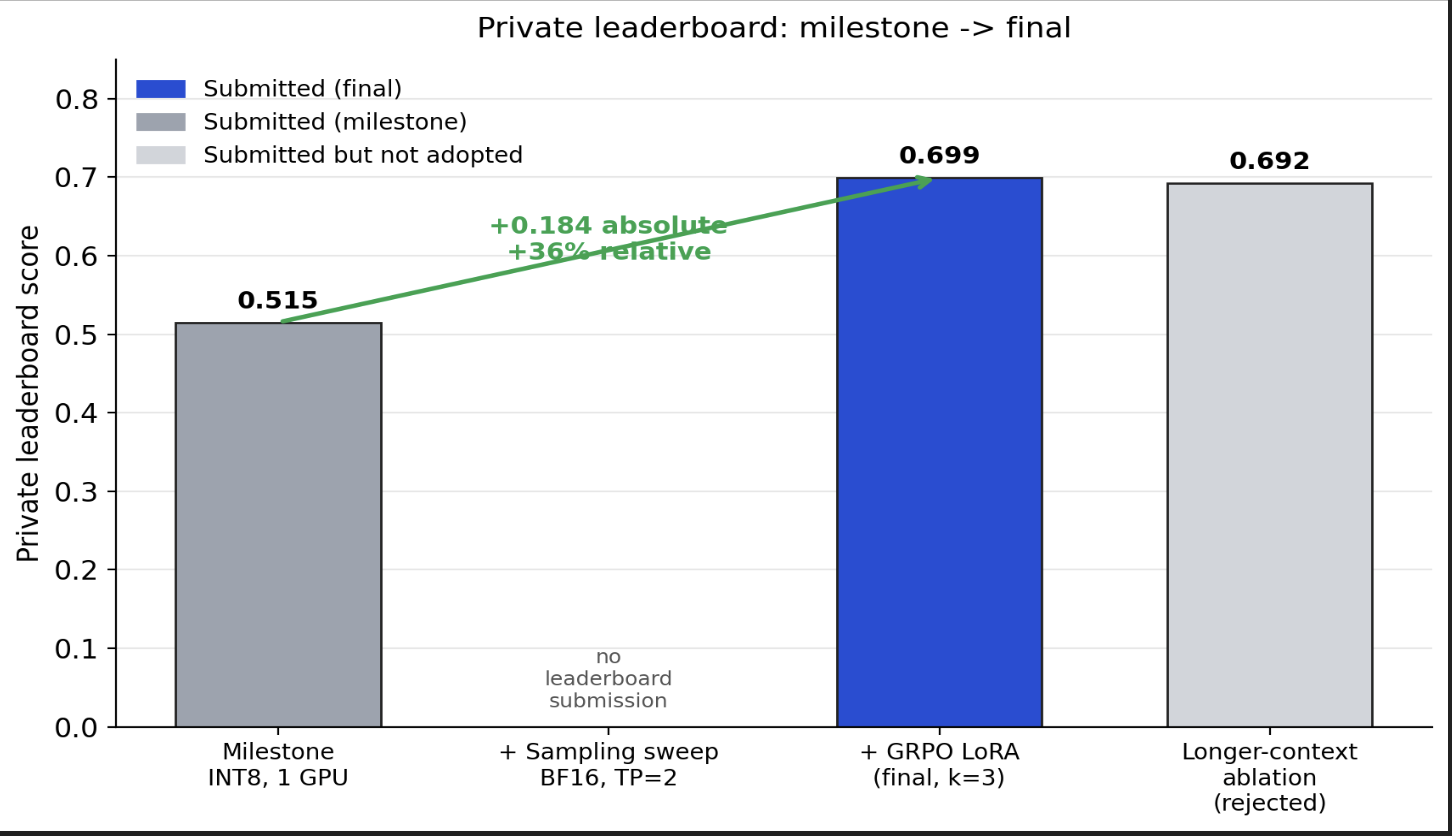
\includegraphics[width=0.75\textwidth]{fig_leaderboard.png}
  \caption{Private-leaderboard progression from the milestone
  submission (INT8, 1 GPU; 0.515 public / 0.459 private) to the
  final submission (BF16 $+$ TP$=2$ $+$ sweep $+$ SC $k{=}3$ $+$
  GRPO LoRA; 0.699 / 0.627), $+0.184$ absolute on the public
  board ($+36\%$ relative). The longer-context ablation submission
  ($0.692$ / $0.612$) is included for reference but was not
  adopted.}
  \label{fig:leaderboard}
\end{figure}

\paragraph{Result 2: $\approx 4.5\times$ inference throughput from INT8 ($1\times$ GPU) to BF16 $+$ vLLM TP$=2$ ($2\times$ A40).}
The milestone pipeline ran Qwen3-4B-Thinking-2507 under INT8
(BitsAndBytes) on a single GPU at $\approx 175$ output
tokens/second. Switching to BF16 weights with vLLM
tensor-parallel $=2$ on $2\times$ A40 raised throughput to
$\approx 786$ tokens/second, roughly $4.5\times$. The reason
quantization was a loss rather than a win is that Qwen3-4B is
only $\approx 8\,$GB in BF16 --- well within a single A40's
$46\,$GB --- so the INT8 path spent most of its budget on
dequantization overhead with no memory headroom to gain. This
change is what made the rest of the final phase tractable: at the
milestone's $\approx 175$ tok/s, a single full-private run at
$k=3$ would have taken $\approx 17$ days instead of the $\approx
4$ it actually took, and we would not have had wall-clock to fit
the sampling sweep, the SC study, and a GRPO training run on top
of it. Figure \ref{fig:throughput} shows the two operating points.

\begin{figure}[h]
  \centering
  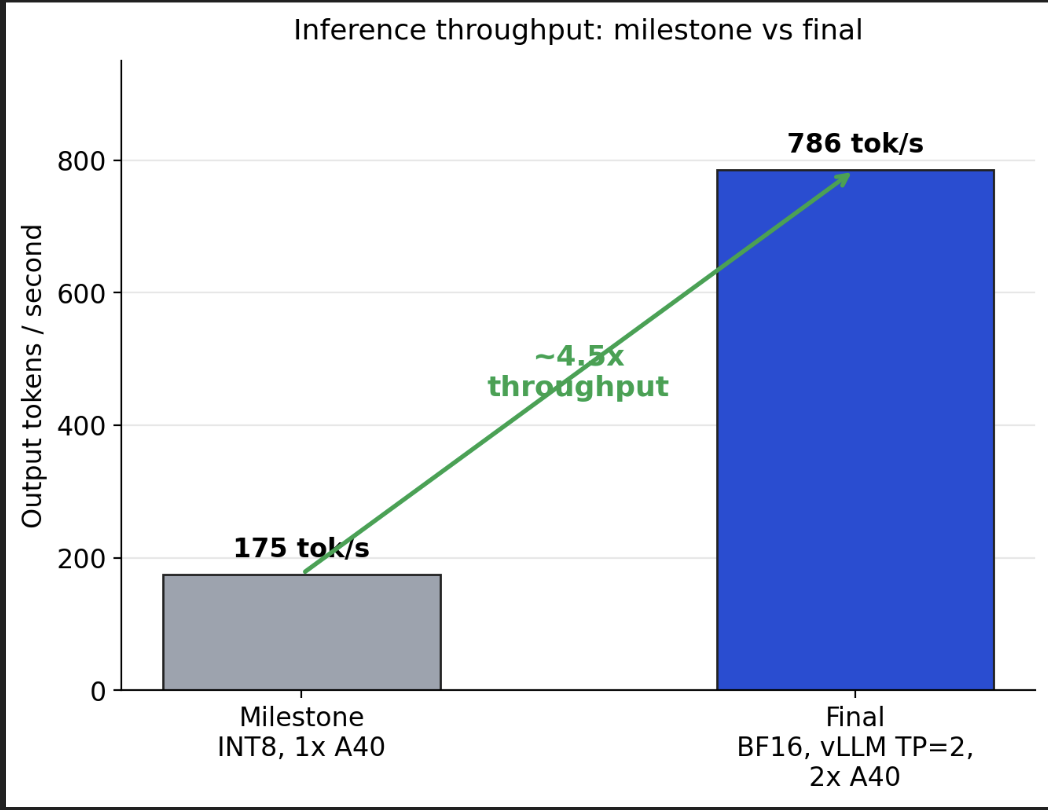
\includegraphics[width=0.55\textwidth]{fig_throughput.png}
  \caption{Output throughput at the milestone (INT8, single A40)
  vs.\ the final pipeline (BF16, vLLM tensor-parallel $=2$ on
  $2\times$ A40), measured during full-private runs. The
  $\approx 4.5\times$ speedup is what made the 24-config sweep, the
  SC study, and one full epoch of GRPO fit in our final-phase
  wall-clock budget.}
  \label{fig:throughput}
\end{figure}


\subsection{Ablations}
\label{sec:ablations}
We isolate the contribution of each component of the final
pipeline by removing or replacing it while holding everything else
fixed. All numbers below are on the 44-item eval slice from
Section \ref{sec:methods} ($10$ MCQ, $34$ free-form), with the
same sampling settings, seeds, and prompt across rows. Table
\ref{tab:eval-slice} gives the layer-by-layer breakdown; the
paragraphs after it isolate each layer in more detail.

\begin{table}[h]
  \caption{Layer-by-layer ablation of the final pipeline on the
  44-item eval slice. All rows use Qwen3-4B-Thinking-2507 under
  BF16 $+$ vLLM TP$=2$ with
  \texttt{(T=0.6, top\_p=0.95, top\_k=20, min\_p=0)}. Each row
  adds one layer to the row above.}
  \label{tab:eval-slice}
  \centering
  \begin{tabular}{lccc}
    \toprule
    Pipeline stage          & MCQ ($n=10$) & Free-form ($n=34$) & Overall ($n=44$) \\
    \midrule
    Sampling sweep (best)                & 80.0\% & 64.7\% & 68.2\% \\
    + Self-consistency ($k=8$)           & 90.0\% & 64.7\% & 70.5\% \\
    + GRPO LoRA                          & 90.0\% & 64.7\% & \textbf{70.5\%} \\
    \bottomrule
  \end{tabular}
\end{table}

\paragraph{Self-consistency size ablation.}
At $k=8$ the vote scored $70.45\%$ overall, identical to the best
single sample on free-form, with a 1-item MCQ swing ($8/10 \to
9/10$) that we treat as noise on a 10-item split. Items the model
gets right were already high-confidence; items it gets wrong
tended to be wrong consistently across rollouts. We dropped $k$
from $8$ to $3$ in the final pipeline --- about $2.7\times$
cheaper at the same expected accuracy on this slice --- and kept
SC as a cheap robustness check rather than a measured gain. The
flatness should be read as ``no signal we can resolve on a slice
this small,'' not ``we proved SC does nothing.''

\paragraph{GRPO adapter ablation.}
On the eval slice the GRPO adapter scored $70.45\%$, identical to
SC alone. Probable causes are listed in Section \ref{sec:methods}:
one low-learning-rate epoch, group size $4$ instead of the
$8$--$16$ from the published recipes, completions truncated at
$2{,}048$ tokens, and a sparse $0/1$ reward. We kept the adapter
in the final pipeline because validation showed no regression on
either the eval slice or the Kaggle leaderboards.

\paragraph{Reasoning-budget ablation.}
We doubled the context budget (\texttt{max\_tokens}
$=16{,}384$, \texttt{max\_model\_len} $=49{,}152$) and re-ran the
final pipeline end-to-end, leaving everything else fixed. The
variant scored $0.692$ public / $0.612$ private --- $-0.007$ on
the public board against the adopted submission's $0.699$. Both
setups use less than $20\%$ of Qwen3-4B-Thinking-2507's
$262{,}144$-token native window, so the KV cache was not the
binding constraint. The wall we are hitting is reasoning
quality, not tokens.


\section{Discussion}
\label{sec:discussion}
We started the final phase from 0.515 public / 0.459 private and
ended at 0.699 public (rank 42/105) / 0.627 private (rank 27/105),
$+36\%$/$+37\%$ relative. The rest of this section
covers what worked, what did not, and what we would try next.

\paragraph{Achievements.}
The pipeline runs end-to-end from a single function call
(\texttt{run\_inference()} in \texttt{run\_inference.py}). The
LoRA adapter is on HuggingFace Hub at
\texttt{k1mittal/cse151b-grpo-lora}, so verification does not
need any local model files. The full 943-item private run
completed with zero empty or errored items after we caught and
fixed the context-budget bug in Section \ref{sec:methods}. On the
eval slice the model's strongest split is MCQ, where the
SC $+$ GRPO pipeline reaches $90\%$ (Table \ref{tab:eval-slice}).

\paragraph{Bottlenecks and Mitigation.}
The sampling sweep was the largest single contribution in the
final phase; SC at $k=8$ and the GRPO adapter were both flat on
the eval slice and we kept them for robustness. The persistent
bottleneck is free-form accuracy, which stayed near $65\%$
through every layer. Inside the free-form split, multi-answer
items (questions wanting a list of values rather than a single
value) were the weakest subset across every method we tried;
our general prompt was not specialized for those items. The
reasoning-budget ablation (Section \ref{sec:ablations}) rules
out token budget as the cause: the wall is reasoning quality,
not tokens. We also did not get through every idea on our list
because of time constraints. From the milestone plan we
deviated in three places: we moved inference from INT8 on one
GPU to BF16 with vLLM TP$=2$ for throughput; we tested SC at
$k=8$ rather than the planned $k\in\{3,5\}$, found no gain, and
shipped $k=3$ for cost; and GRPO ran with reduced group size
and shorter completions because of single-box memory.

\paragraph{Lessons Learned.}
\begin{itemize}
    \item \textbf{Run small eval chunks before full runs.}
    Running each change on a small chunk of the public set first
    gave us a clean read on whether the change was actually
    helping the model, without paying for a full-private run on
    every experiment.
    \item \textbf{Use overnight runs to parallelize work.}
    Wrapping the notebook in bash scripts and letting it run
    overnight on the remote server meant we could keep
    experiments going in the background while we worked on
    other things, which gave us back a lot of wall-clock time.
    \item \textbf{If given more time.} (i) Use the model's
    context tokens better and write prompts that target the
    multi-select questions specifically, where our general
    prompt left accuracy on the table; (ii) augment GRPO
    fine-tuning with NVIDIA's Nemotron dataset to strengthen the
    post-training stage.
\end{itemize}

\paragraph{Team Responsibilities.}
\begin{itemize}
    \item \textbf{Ketan Mittal} --- grader analysis, prompt
    design, sampling-parameter sweep, final private run,
    bug-fixes, and the submission pipeline.
    \item \textbf{Anirudh Annabathula} --- inference
    infrastructure (vLLM TP$=2$, BF16 on $2\times$A40), GRPO
    training setup on the GPUs, and the presentation.
    \item \textbf{Kaii Bijlani} --- dataset analysis, the
    Claude-based answer filter over the public set, and the
    presentation.
\end{itemize}


\section*{LLM Usage}
We used an LLM assistant (Anthropic Claude) for two things in the
report-writing process: (i) help with wording, mostly tightening
up phrasing in this report and in our system prompts, and
(ii) help making sense of hard-to-read error messages in LaTeX
and Python while we were writing the report and building the
pipeline. We also used Claude as a \emph{verifier} for the GRPO
training set --- it read each public-set item and flagged ones
whose published gold answer was wrong or ambiguous --- which is
methodological use rather than report-writing assistance, and is
described as such in Section \ref{sec:methods}. All the technical
decisions, code, experimental runs, and numbers in this report
are ours.


\bibliography{references.bib}
\bibliographystyle{plainnat}

\end{document}
